\section{Blockchain und Internet of Things}
Die Blockchain-Technologie bringt bereits einige Vorteile für Finanzsektor mit sich.
In der Kombination mit Internet of Things (IoT) lassen sich einige der bereits erörterten Einsatzgebiete
für breitere Anwendungsmöglichkeiten erweitern.
% IoT 
% kurz, dass ioT Daten sammeln können, die in der Blockchian gespeichert werden können und in Smart Contracts
% verarbeitet werden können

\subsection{Anwendungsmöglichkeiten/Synergien mit Internet of Things}

\subsubsection{Lieferkettenfinanzierung}
Integriert man IoT-Sensoren mit einer Blockchain-Struktur, können in der Lieferkette Zeit und Kosten bei
jeder Übergabe eingespart werden.
% Asset Tracking
Die IoT-Technologie schafft die Möglichkeit für Asset Tracking, um den Zustand von physischen Assets
kontinuierlich einsehen zu können. Durch das Anbringen von internetfähigen Sensoren an 
Liefercontainern kann so der Status des Transports vollumfänglich transparent gestaltet
werden und in Echtzeit abgefragt werden. 
Informationen die hierbei von Interesse sind, wären der aktuelle Standort der Lieferung und
die vorraussichtliche Ankunftszeit. Erweiternd dazu kann für empfindliche und 
verderbliche Waren die Temperatur, Luftfeuchtigkeit oder starke Erschütterungen auf dem 
Transportweg aufgezeichnet werden.
% Speichern und Smart Contract
Die Blockchain-Technologie bietet die Funktionalität, die erfassten Informationen in Blöcken
zu speichern. Damit fungiert die Blockchain wie ein Transportbericht der gesamten Lieferkette und 
sichert nebenbei die Integrität und Richtigkeit der Daten, sofern keine Sensorprobleme vorliegen. 
Zusätzlich kann bei der Zustellung der Lieferung ein Smart Contract die Zahlung automatisch durchführen.
So werden der Zeitaufwand und die Kosten für Qualitätsprüfungen reduziert und vor allem verderbliche 
Waren können schneller weiterverarbeitet werden.
\cite[p.~169f]{chowdhary2025smart}


\subsubsection{Risiko-Management}
\label{sec:Risk_Management}
Der kontinuierliche Datenstrom von IoT-Sensoren kann zur Risikobewertung hergenommen werden.
Die Auswertung dieser Daten kann im Nachgang zur Eingrenzung potentieller Schäden 
verwendet werden.
Versicherungsunternehmen können die Daten aus einem Auto verwenden, sofern es beispielsweise
eine Car2Car-Kommunikation besitzt, um die Beiträge an das individuelle Fahrverhalten
anzupassen. 
Wenn die Sensoren oft einen riskanten Fahrstil melden, wie Geschwindigkeitsüberschreitungen oder 
nicht-einhalten von Mindestabständen, kann der Beitrag für die einzelne Person erhöht werden. Auf der 
Gegenseite kann sicheres Fahren mit niedrigeren Beiträgen belohnt werden. 
Dadurch ermutigt das Unternehmen zu einem vorsichtigeren Fahrstil, woraus weniger Unfälle resultieren 
können und daraus folgernd weniger Versicherungsansprüche gestellt werden.
\cite[p.~169f]{chowdhary2025smart}
Eine Anpassung des Beitrags kann ggf. erst nach längerem Beibehalten des Fahrstils automatisch mit einem 
Smart Contract vorgenommen werden.

Eine weitere Form Risiken einzugrenzen ist vorausschauendes Risiko-Management, welches die 
Betriebseffizienz steigern soll.
Eine mögliche Anwendung kann daraus bestehen, einen Leistungsbericht von Maschinen in einer Produktionskette
zu erstellen. IoT-Sensoren können hierfür einen kontinuierlichen Datenstrom als Basis für den Bericht liefern.
Aus dem Bericht können nachfolgen Leistungsschwankungen und -einbrüche erkannt werden und frühzeitig 
Gegenmaßnahmen eingeleitet werden. Dadurch können Ausfälle der Produktionskette und damit einhergehende 
finanzielle Schäden minimiert werden.
\cite[p.~169]{chowdhary2025smart}

% Kreditrisiko in der Lieferkette \cite[p.~347ff]{Zhang2021Research}




\subsubsection{Smart Contracts und IoT}
% IoT Device Administration
Smart Contracts bieten die Möglichkeit die Geräteverwaltung von IoTs zu automatisieren und zu dezentralisieren.
Mittels einer Blockchain kann ein System konstruiert werden, welches die Kommunikation zwischen IoT-Geräten
durch Blöcke realisiert. 
Vergleichsweise wird in zentralen Strukturen immer ein Intermediär benötigt, der beispielsweise ein 
Update-Request von einem Gerät A an ein Gerät B weiterleitet, welches dann das Update vornimmt.

Eine derartige Kommunikationsstruktur kann wie in \autoref{fig:SC-IoT_Update} dargestellt, umgesetzt werden.
Im ersten Schritt (1) schickt Device A einen Smart Contract an die Blockchain. Die Miner validieren diesen
und fügen den Contract in einem neuen Block hinzu (2 - 3). Dadurch besitzen alle Geräte, die Teil dieser 
Struktur sind, eine lokale Kopie des Smart Contract mit der Update-Funktion (4 - 5).
Nach der Verteilung der Daten ruft Gerät A die Update-Funktion in einer neuen Transaktion auf, welche 
wieder von den Minern in einem weiteren Block bestätigt wird (6 - 7). 
Der Smart Contract fügt bei der Ausführung einen dritten Block hinzu (8). Dieser beinhaltet ein Event,
welches den Update-Prozess auslöst.
Alle IoT-Geräte in diesem Netzwerk registrieren das Event und rufen die zugehörige Funktionalität auf, was
das Update durchführt (9). 
Anschließend schicken sie eine Bestätigung mit ihrem Status des Updates an das Netzwerk (10 - 11).

Auf diese Weise können Firmware-Updates und andere Software-Erweiterungen mit geringem Organisationsaufwand auf allen 
Geräten durchgeführt werden. 
Auch Geräte-spezifische Funktionalitäten eines IoT können so von einem anderen Gerät aufgerufen werden.
Dieser Ablauf ist einfach skalierbar, da der Datenaustausch über Broadcasts stattfindet.  
Dadurch können beliebig viele IoT-Geräte dem Netzwerk hinzugefügt werden ohne den Kommunikationsaufwand 
proportional zu erhöhen. 
Zusätzlich sichern die Eigenschaften der Blockchain die Transparenz, Datenintegrität und Sicherheit der
Authentifizierung dieses Prozesses.
%Zusätzlich ist dieser Prozess durch die Eigenschaften der Blockchain transparent, 
\cite[p.~74f]{Choi2018DeviceControl}


% Wartungen von anderen Geräten (Smarte Geldautomaten)
Smart Contracts können auch zur Planung und Koordinierung von Wartungen oder Steigerung der Betriebseffizienz 
verwendet werden.
Wie im Kapitel \ref{sec:Risk_Management} erklärt, können Leistungsberichte von IoT-Geräten erstellt werden.
Durch eine Erweiterung um Smart Contracts kann der Anstoß zum Wartungsprozess automatisiert werden. Bei einem
festen Vertragspartner, welcher diese durchführt, kann sogar der gesamte Prozess automatisiert werden. 
Der Contract kann bei der Ausführung eine Buchung zum nächstmöglichen Termin auslösen und bei Erfüllung 
der Wartung automatisch die Kosten begleichen.
\cite[p.~169ff]{chowdhary2025smart}

% Smart Contracts und IoT
\begin{figure}[!h]
    \begin{center}
        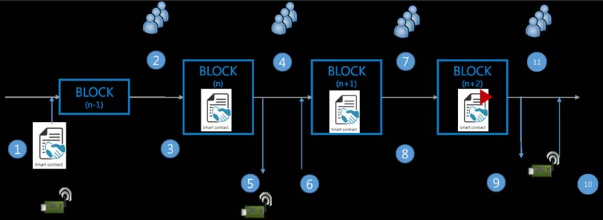
\includegraphics[height=5cm]{SC-IoT_Updating.png}
    \end{center}
    \quelle{\cite[p.~75]{Choi2018DeviceControl}}
    \caption{Kommunikation zwischen IoTs mithilfe von Smart Contracts}
    \label{fig:SC-IoT_Update}
\end{figure}



\subsubsection{Asset Tokenization}


\subsubsection{Analyse von Nutzerverhalten}

% Smart Wearables

% Fraud Detection


\subsection{Ausblick und Risiken}

% Chentara: Daten von Versicherungen und sonstige gespeicherte Daten sind öffentlich nur als Hashes einsehbar
% -> kein Rückschluss auf die eigentlichen Datenwerte möglich